\documentclass{standalone}
\input{feynman_settings}

\definecolor{gold}{rgb}{0.83, 0.69, 0.22}
\definecolor{auburn}{rgb}{0.43, 0.21, 0.1}

\begin{document}
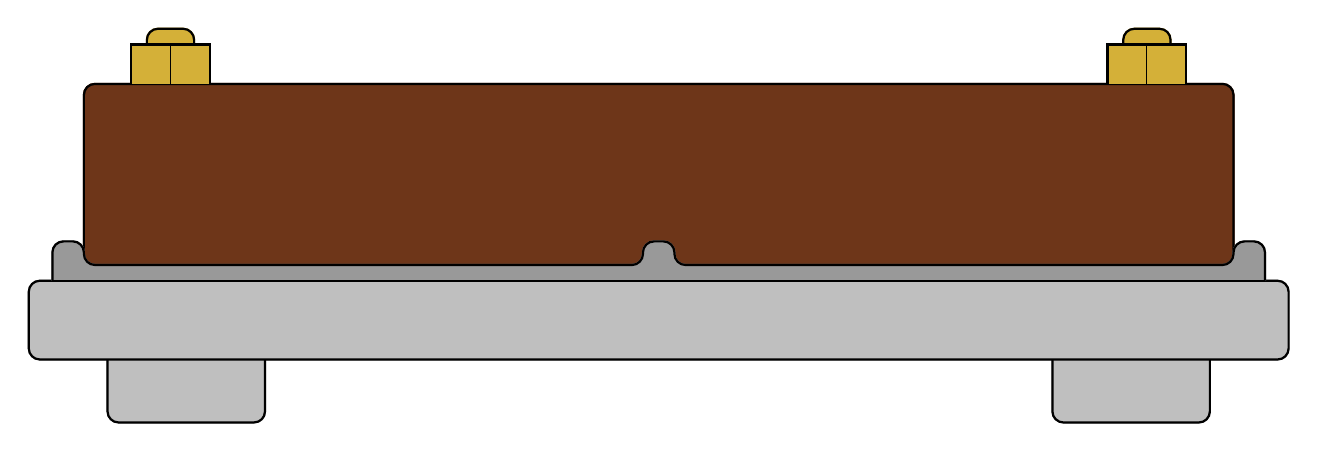
\begin{tikzpicture}

%Grid zum pr�ziseren Arbeiten
%\draw[help lines, thin, dashed] (-9,-3) grid (9,3);
	
%F�llung Metalplatten	
\filldraw[thick, rounded corners, gray!50!white] (-7.8,-2) -- (8,-2) -- (8, -1) -- (-8,-1) -- (-8,-2) -- (-7.7,-2);
\filldraw[thick, rounded corners, gray!50!white] (-7, -2) -- (-7, -2.8) -- (-5, -2.8) -- (-5, -2);
\filldraw[thick, rounded corners, gray!50!white] (7, -2) -- (7, -2.8) -- (5, -2.8) -- (5, -2);
	

%Metallplatte unten
\draw[thick, rounded corners] (-7.8,-2) -- (8,-2) -- (8, -1) -- (-8,-1) -- (-8,-2) -- (-7.7,-2);

%F��e Metallplatte	
\draw[thick, rounded corners] (-7, -2) -- (-7, -2.8) -- (-5, -2.8) -- (-5, -2);

\draw[thick, rounded corners] (7, -2) -- (7, -2.8) -- (5, -2.8) -- (5, -2);

%Bauteil
\filldraw[thick, rounded corners, auburn] (-7.1,-0.8) -- (7.3,-0.8) -- (7.3, 1.5) -- (-7.3,1.5) -- (-7.3,-0.8) -- (-7.1,-0.8);
\draw[thick, rounded corners] (-7.1,-0.8) -- (7.3,-0.8) -- (7.3, 1.5) -- (-7.3,1.5) -- (-7.3,-0.8) -- (-7.1,-0.8);

%Schrauben
\filldraw[thick, gold] (-6.7, 1.5) -- (-6.7,2) --  (-5.7,2) -- (-5.7,1.5);
\filldraw[thick, rounded corners, gold] (-6.5, 2) -- (-6.5, 2.2) -- (-5.9, 2.2) -- (-5.9,2) ;
\draw[thick] (-6.7, 1.5) -- (-6.7,2) --  (-5.7,2) -- (-5.7,1.5);
\draw[thin] (-6.2, 2) -- (-6.2,1.5);
\draw[thick, rounded corners] (-6.5, 2) -- (-6.5, 2.2) -- (-5.9, 2.2) -- (-5.9,2) ;

\filldraw[thick, gold] (6.7, 1.5) -- (6.7,2) --  (5.7,2) -- (5.7,1.5);
\filldraw[thick, rounded corners, gold] (6.5, 2) -- (6.5, 2.2) -- (5.9, 2.2) -- (5.9,2) ;
\draw[thick] (6.7, 1.5) -- (6.7,2) --  (5.7,2) -- (5.7,1.5);
\draw[thin] (6.2, 2) -- (6.2,1.5);
\draw[thick, rounded corners] (6.5, 2) -- (6.5, 2.2) -- (5.9, 2.2) -- (5.9,2) ;

%Halterung 
\filldraw[thick, rounded corners, gray!80!white] (-7.7,-1) -- (-7.7, -0.5) -- (-7.3,-0.5) -- (-7.3, -0.8) -- (-0.2, -0.8) -- (-0.2, -0.5) -- (0.2, -0.5) -- (0.2, -0.8) -- (7.3, -0.8) -- (7.3, -0.5) -- (7.7, -0.5) -- (7.7, -1);
\draw[thick, rounded corners] (-7.7,-1) -- (-7.7, -0.5) -- (-7.3,-0.5) -- (-7.3, -0.8) -- (-0.2, -0.8) -- (-0.2, -0.5) -- (0.2, -0.5) -- (0.2, -0.8) -- (7.3, -0.8) -- (7.3, -0.5) -- (7.7, -0.5) -- (7.7, -1);
\draw[thick] (7.7, -1) -- (-7.7, -1);


	
\end{tikzpicture}
\end{document}